\documentclass[]{article}
\usepackage{amsmath}
\usepackage{graphicx}
\graphicspath{ {imgs/} }

%opening
\title{ADIPCV Assignment IV}
\author{}

\begin{document}

\maketitle

For instructions regarding running code, kindly refer to the \texttt{README.md} file attached.

\section{Color Correction}
The color is corrected for the images using Gray World and White World approximation
algorithms. $\alpha$ and  $\beta$ are calculated as follows and scaled accordingly
for the target images. For White World,
\begin{equation}
  \alpha = \frac{g_{max}}{r_{max}}, \beta = \frac{g_{max}}{b_{max}}
\end{equation}

and for Gray World,
\begin{equation}
  \alpha = \frac{g_{mean}}{r_{mean}}, \beta = \frac{g_{mean}}{b_{mean}}
\end{equation}

\begin{figure}[h!]
  \begin{center}
    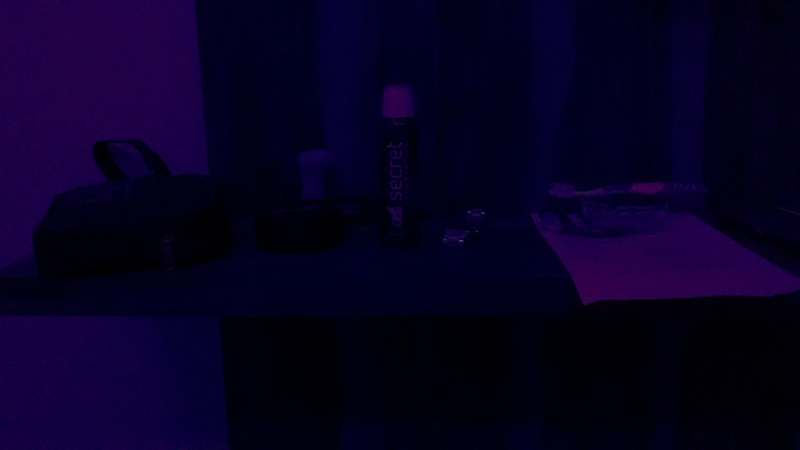
\includegraphics[scale=0.4]{self_recons_artificial}
    \caption[p3]{Color Corrected Artificial Image}
  \end{center}
\end{figure}
\begin{figure}[h!]
  \begin{center}
    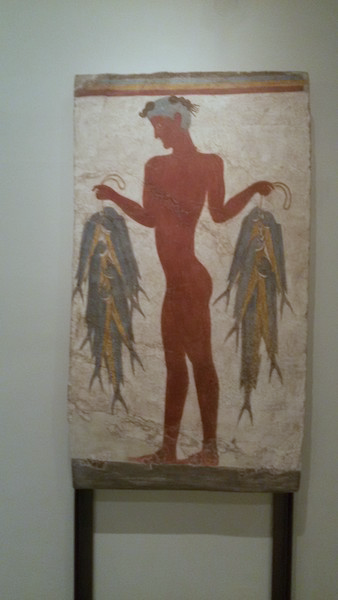
\includegraphics[scale=0.4]{self_recons_thera}
    \caption[p3]{Color Corrected Wall Painting}
  \end{center}
\end{figure}
\section{Saturation of the Image}
The gamut triangle is calculated for the images by tranforming it from the RGB to the XYZ space.
Also, ${x,y}$ are calculated by normalization. The position of the maximally saturated point is the
extended point of the corresponding image point on the triangle line. This is determined by finding
the corresponding triad in which the point is present with respect to $\mathbf{W}(0.33, 0.33)$.

The functions are implemented in a modular fashion, reusing line and intersection implementations
from earlier assignments.

For further saturating the image by an amount $k$, the image is mapped further to a smaller gamut triangle
depending upon taking a point $k:1$ using section formula, where $k=\infty$ corresponds to the maximally
saturated image.

Some of the gamut triangles are shown below:
\begin{figure}[h!]
  \begin{center}
    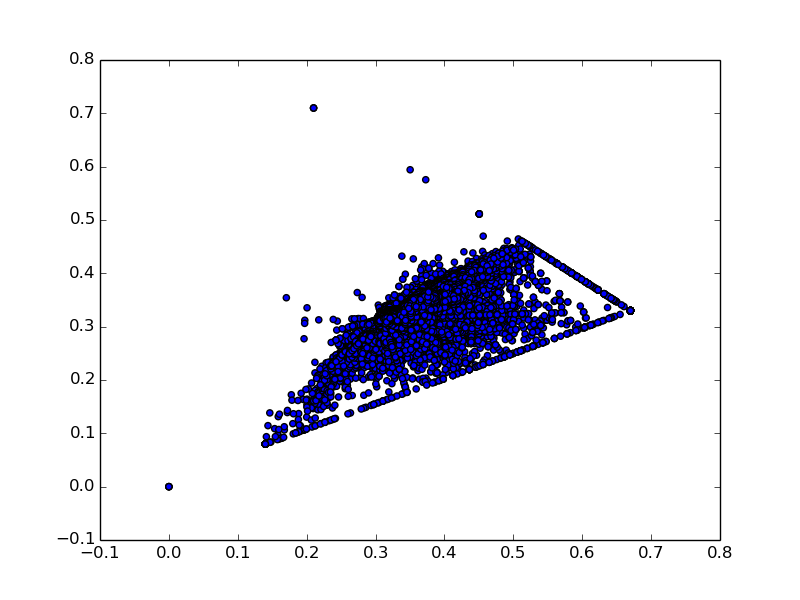
\includegraphics[scale=0.4]{gamut_trianglenormal}
    \caption[p1]{Original Gamut Triangle}
  \end{center}
\end{figure}
\begin{figure}[h!]
  \begin{center}
    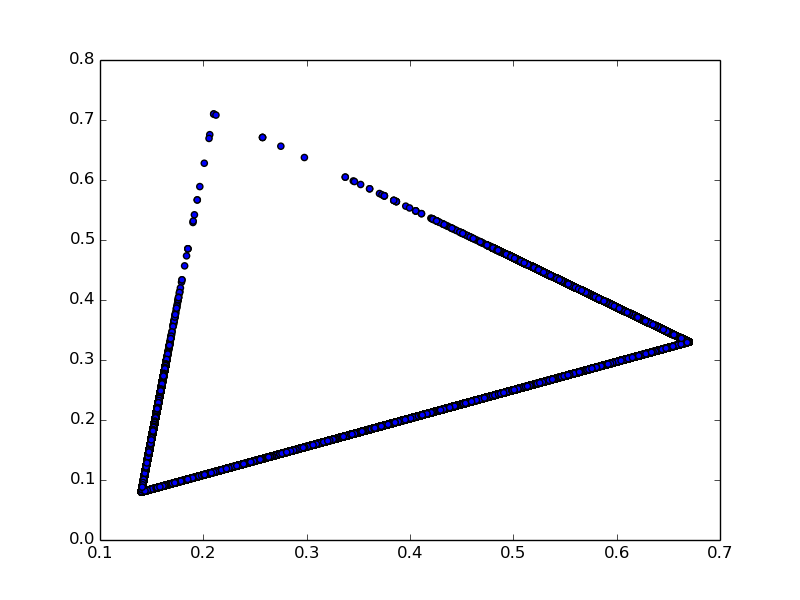
\includegraphics[scale=0.4]{gamut_triangle_maxsat_normal_100}
    \caption[p1]{Gamut Triangle for k = 100}
  \end{center}
\end{figure}
\begin{figure}[h!]
  \begin{center}
    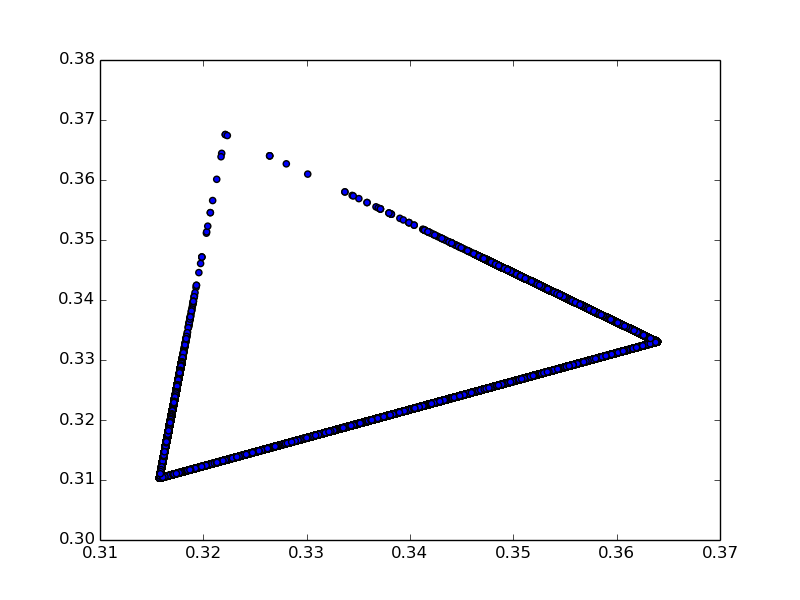
\includegraphics[scale=0.4]{gamut_triangle_maxsat_normal_0_1}
    \caption[p2]{Gamut Triangle for k = 0.1}
  \end{center}
\end{figure}
\begin{figure}[h!]
  \begin{center}
    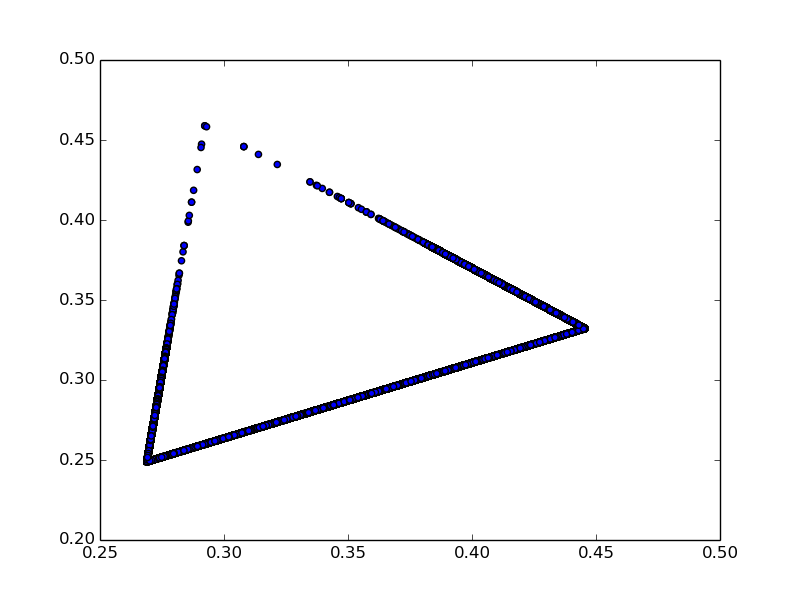
\includegraphics[scale=0.4]{gamut_triangle_maxsat_normal_0_5}
    \caption[p3]{Gamut Triangle for k = 0.5}
  \end{center}
\end{figure}

\begin{figure}[h!]
  \begin{center}
    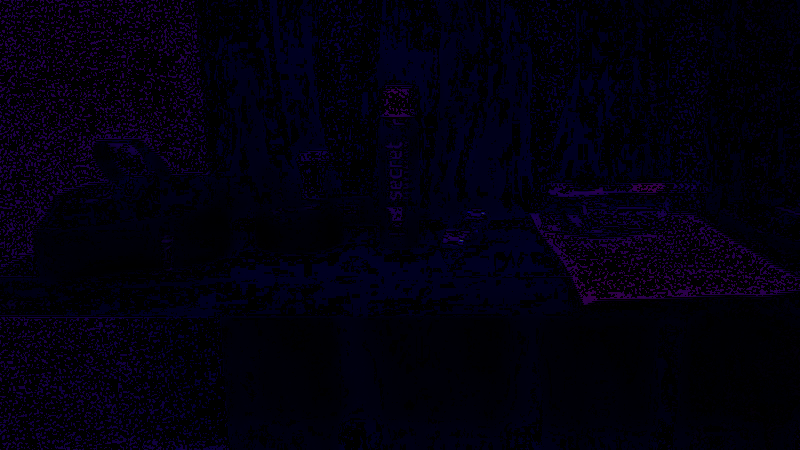
\includegraphics[scale=0.4]{recons_100_artificial}
    \caption[p3]{Maximally Saturated Artificial Image}
  \end{center}
\end{figure}
\begin{figure}[h!]
  \begin{center}
    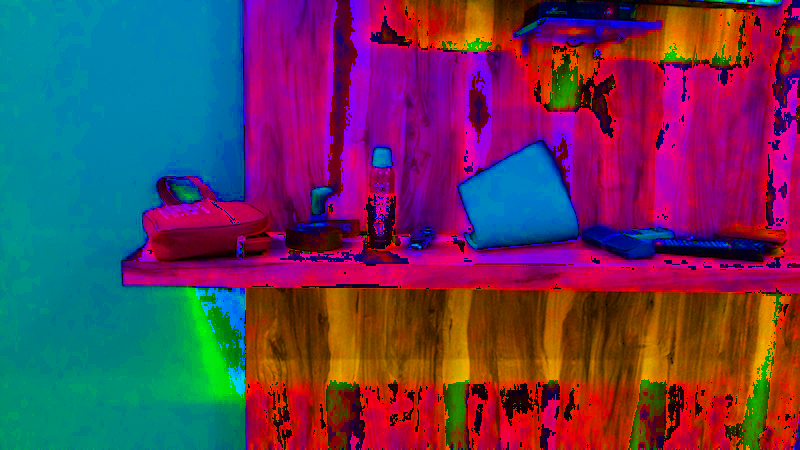
\includegraphics[scale=0.4]{recons_100_normal}
    \caption[p3]{Maximally Saturated Normal Image}
  \end{center}
\end{figure}
\begin{figure}[h!]
  \begin{center}
    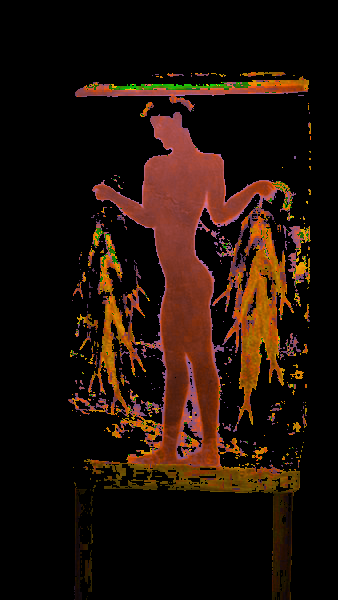
\includegraphics[scale=0.4]{recons_100_thera}
    \caption[p3]{Maximally Saturated Wall Painting}
  \end{center}
\end{figure}

Some of the best saturation levels are shown below:
\begin{figure}[h!]
  \begin{center}
    \includegraphics[scale=0.4]{recons_0_3_artificial}
    \caption[p3]{Best Image for Artificial Image with k=0.3}
  \end{center}
\end{figure}
\begin{figure}[h!]
  \begin{center}
    \includegraphics[scale=0.4]{recons_0_1_normal}
    \caption[p3]{Best Image for Normal Image with k=}
  \end{center}
\end{figure}
\begin{figure}[h!]
  \begin{center}
    \includegraphics[scale=0.4]{recons_0_7_thera}
    \caption[p3]{Best Image for Wall Painting k=}
  \end{center}
\end{figure}

\end{document}
